\section{Linear elasticity equations}

Linear elasticity is a mathematical model of the behavior of solids and describes the internal stress state under the influence of small deformations. A simplified model of a more complete theory of nonlinear elasticity and a section on the mechanics of solid bodies. The main assumption is that the deformations are small and the generalized Hooke's law applies. This problem was chosen to demonstrate the method, since it is often used in conjunction with filtration models, and poroelastic media models are used. If it is possible to solve the proposed problem with high accuracy of approximation, then it will be possible to use this approach to simulate more complex processes, such as hydraulic fracturing.

The system of equations for the linear elasticity problem is as follows:
\begin{equation}
	\label{eq:linear_sys}
	\begin{cases}
		- \nabla \sigma = f \\[10pt]
		\sigma = \lambda \epsilon_v I + 2 \mu \epsilon, \quad \epsilon_v = Tr \left ( \epsilon \right ) \\[10pt]
		\epsilon = \dfrac{1}{2} \left [ \nabla u + \left ( \nabla u\right )^T \right ] \\[10pt]
		u = \vec{u} = \left [ u_x, u_y \right ]^T, \quad \vec{x} = (x, y) \in \Omega \subset R^2
	\end{cases}
\end{equation}
More detailed explanation available here \cite{barber1992elasticity}, \cite{gould1983introduction}.
In component form, the system of equations looks like this:
\begin{center}
	\begin{equation}
		\begin{split}
			\nabla u = \begin{pmatrix}
			\dfrac{\partial }{\partial x} \\[10pt]
			\dfrac{\partial }{\partial y}
			\end{pmatrix} \begin{pmatrix}
			u_x & u_y
			\end{pmatrix} = \begin{pmatrix}
			\dfrac{\partial }{\partial x} u_x & \dfrac{\partial }{\partial x} u_y \\[10pt]
			\dfrac{\partial }{\partial y} u_y & \dfrac{\partial }{\partial y} u_y 
			\end{pmatrix}, 
			- \nabla \sigma = -\nabla \left [ \lambda \epsilon_v I + 2 \mu \epsilon \right ] = \\[10pt] = \lambda \begin{pmatrix}
			 \dfrac{\partial }{\partial x} \dfrac{\partial }{\partial x} u_x + \dfrac{\partial }{\partial x} \dfrac{\partial }{\partial y} u_y \\[10pt]
			 \dfrac{\partial }{\partial y} \dfrac{\partial }{\partial x} u_x + \dfrac{\partial }{\partial y} \dfrac{\partial }{\partial y} u_y
			\end{pmatrix} + \mu \begin{pmatrix}
			2 \dfrac{\partial }{\partial x} \dfrac{\partial }{\partial x} u_x  + \dfrac{\partial }{\partial y} \dfrac{\partial }{\partial y} u_y + \dfrac{\partial }{\partial y} \dfrac{\partial }{\partial x} u_y \\[10pt]
			\dfrac{\partial }{\partial x} \dfrac{\partial }{\partial x} u_y + \dfrac{\partial }{\partial x} \dfrac{\partial }{\partial y} u_y + 2 \dfrac{\partial }{\partial y} \dfrac{\partial }{\partial y} u_y 
			\end{pmatrix}
			\implies \\[10pt] \begin{cases}
			\lambda \left [ \dfrac{\partial }{\partial x} \dfrac{\partial }{\partial x} u_x + \dfrac{\partial }{\partial x} \dfrac{\partial }{\partial y} u_y \right ] + \mu \left [ 2 \dfrac{\partial }{\partial x} \dfrac{\partial }{\partial x} u_x  + \dfrac{\partial }{\partial y} \dfrac{\partial }{\partial y} u_y + \dfrac{\partial }{\partial y} \dfrac{\partial }{\partial x} u_y \right ] = -f_x \\[10pt]
			\lambda \left [ \dfrac{\partial }{\partial y} \dfrac{\partial }{\partial x} u_x + \dfrac{\partial }{\partial y} \dfrac{\partial }{\partial y} u_y \right ] + \mu \left [ \dfrac{\partial }{\partial x} \dfrac{\partial }{\partial x} u_y + \dfrac{\partial }{\partial x} \dfrac{\partial }{\partial y} u_y + 2 \dfrac{\partial }{\partial y} \dfrac{\partial }{\partial y} u_y  \right ] = -f_y
			\end{cases}
		\end{split}
	\end{equation}
\end{center}
And so, the system of equations is described. The boundary conditions are as follows:
\begin{equation}
	\vec{n} \cdot \vec{u} = U, \forall \vec{x} \in \partial \Omega_u, \quad \vec{n} \cdot \sigma = \vec{T}, \forall \vec{x} \in \partial \Omega_T
\end{equation}

Similarly, as for the Stokes equations, computational experiments will be carried out for different architectures. A study will also be conducted on the effect of the activation function on the quality of the solution. Model architectures will be defined as \eqref{eq:neural_net_by_vec}, table \ref{table:linear_tab} describes all configurations to consider. Problem \eqref{eq:linear_sys} is considered inside a rectangular region, with boundary conditions:
\begin{equation}
	\label{eq:boundary_conditions}
	\begin{cases}
		u_x = 0.1, \quad x = 0 \\
		u_x = -0.1, \quad x = 1 \\
		u_y = 0.1, \quad y = 0 \\
		u_y = 0.0, \quad y = 1 \\
	\end{cases}
\end{equation}

\begin{figure}
	\centering
	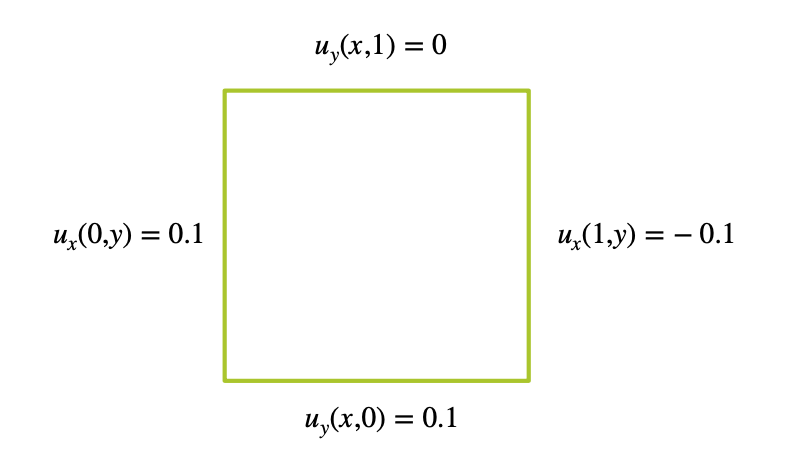
\includegraphics[width=\textwidth]{images/chapter3/linear_description.png}
	\caption{$\Omega$ and boundary conditions from \eqref{eq:boundary_conditions}}
	\label{fig:linear_description}\tabularnewline
\end{figure}

\begin{table}
	\centering
	\begin{tabular}{| c | c | c |} 
	\hline
		$\vec{n}$ & Parameters number & Accuracy \\ \hline
		$[2, 4, 3]$ & 20 & $0.00021$ \\ \hline
		$[2, 8, 3]$ & 40 & $0.00007$ \\ \hline
		$[2, 16, 3]$ & 70 & $0.00002$ \\ \hline
		$[2, 4, 4, 3]$ & 36 & $0.00016$ \\ \hline
		$[2, 8, 8, 3]$ & 104 & $0.000014$ \\ \hline
		$[2, 16, 16, 3]$ & 334 & $0.00001$ \\ \hline
	\end{tabular}
	\caption{Accuracy of the solution for different number of the parameters [Linear elasticity]}
	\label{table:linear_tab}
\end{table}

Table \ref{table:linear_tab} describes the structures of the models on which the experiment will be conducted. To assess the optimal structure, figure \ref{fig:linear_param_vs_accuracy} will be used, showing the results of table \ref{table:linear_tab}.

\begin{figure}
	\centering
	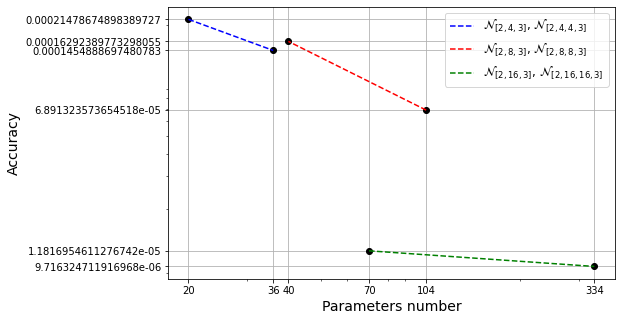
\includegraphics[width=\textwidth]{images/chapter3/linear_param_vs_accuracy.png}
	\caption{Parameters number vs Accuracy, description of the table \ref{table:linear_tab}}
	\label{fig:linear_param_vs_accuracy}\tabularnewline
\end{figure}

 The solution to problem \eqref{eq:linear_sys} is the function $u$, which describes the field of displacements of elementary volumes, the description \cite{barber1992elasticity}.

\begin{figure}
	\centering
	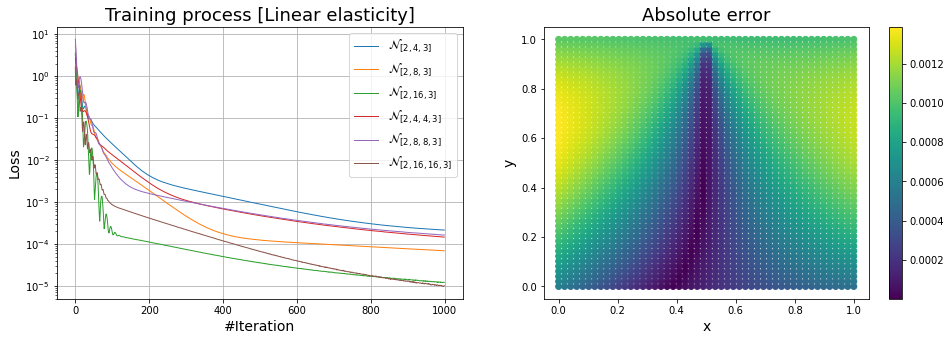
\includegraphics[width=\textwidth]{images/chapter3/linear_simple_net_train_error.png}
	\caption{Parameters number vs Accuracy, description of the table \ref{table:linear_tab}}
	\label{fig:linear_simple_net_error_train}\tabularnewline
\end{figure}

It can be seen from figure \ref{fig:linear_param_vs_accuracy}, \ref{fig:linear_simple_net_error_train} that an increase in depth does not lead to such a strong solution quality as an increase in the network width, moreover, in terms of the computational complexity of the algorithm, it becomes clear that it is optimal to use no more than 2-3 layers, then the quality increase for the required computational costs getting small. In fact, it’s not particularly important to try to use other activation functions, it’s important that for the given tasks it’s already becoming clear that the work describing neural networks with hundreds or even thousands of parameters is exhaustively large for such tasks, since it is clear that for systems of equations that although they are solved analytically, they are still quite complicated. It is also worth noting the connection between the availability of an analytical solution and the required number of parameters for solving problems.

\begin{figure}
	\centering
	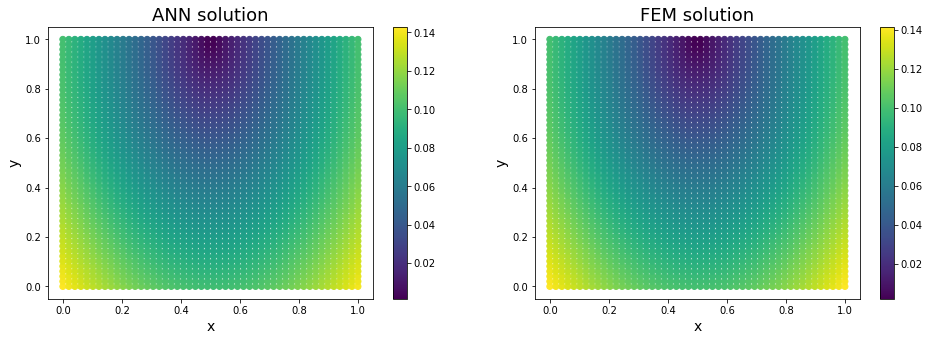
\includegraphics[width=\textwidth]{images/chapter3/linear_simple_net_solution.png}
	\caption{Solution for the \eqref{eq:linear_sys}}
	\label{fig:linear_simple_net_error_train}\tabularnewline
\end{figure}